% !TeX encoding = UTF-8
% !TeX spellcheck = es_ES
% !TeX root = ComponentCatalog.tex
%!TEX root=ComponentCatalog.tex

\documentclass[spanish]{DccDiyTools/DccDiyTools}
\usepackage[spanish]{babel}
\usepackage[
type={CC},
modifier={by-sa},
version={4.0},
]{doclicense}

\usepackage[]{DccDiyTools/DccDiyToolsPics}
\usepackage[]{DccDiyTools/DccDiyToolsComponentTables}

\title{Catalago de Componentes}
\subtitle{Componentes usado en DccDiyTools}
\author{Daniel Vilas}
\date{Julio 2022}

\dbType{M}
\dbDate{22}
\dbCode{001}
\dbStatus{Draft}
\dbVersion{0.1}
%\tikzset{
    pics/SmallBoard/.style={
      code = {
        % \draw [step=0.1,very thin, yellow] (-2,-1) grid (2,1);
        % \draw [step=0.5,very thin, red] (-2,-1) grid (2,1);
        % \draw [very thin, green] (-2,-1) grid (2,1);
        \node[inner sep=0pt] at (0,0)
        {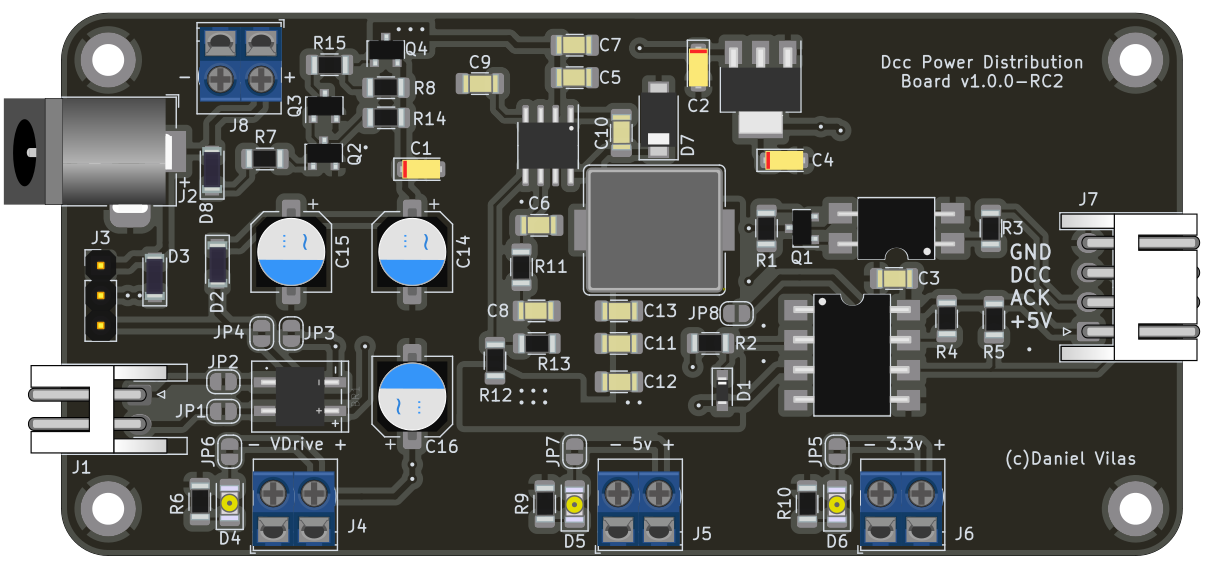
\includegraphics[scale=0.25]{images/front.png}};  


        \node[](-jack) at (-1.35,0.278) {};
        \node[](-terminal) at (-.8,0.65) {};
    }}
}

\tikzset{
    pics/WallAc/.style={
      code = {
    \begin{scope}[shift={(0.25,0)}]
        % \draw [step=0.1,very thin, yellow] (-2,-2) grid (2,2);
        % \draw [step=0.5,very thin, red] (-2,-2) grid (2,2);
        % \draw [very thin, green] (-2,-2) grid (2,2);
        % Mains lead
        \draw[line width=2pt,cap=round, lightgray] (0.05,-0.21) -- (0.05,-0.45);
        \draw[line width=2pt,cap=round, lightgray] (0.275,-0.21) -- (0.275,-0.45);
        % Relief and out cable
        \draw[line width=2pt,cap=round] (-0.5,0.25) -- (-1,0.25);
        \draw[line width=2pt,cap=round,black!75] (-0.55,0.35)--(-0.55,0.15);
        \draw[line width=2pt,cap=round,black!75] (-0.63,0.325)--(-0.63,0.175);
        \draw[line width=2pt,cap=round,black!75] (-0.71,0.3)--(-0.71,0.2);
        \draw[line width=2pt,cap=round,black!75] (-0.79,0.275)--(-0.79,0.225);
        \draw[line width=2pt,cap=round,black!75] (-0.87,0.275)--(-0.87,0.225);

        \draw[line width=2pt,rounded corners=1pt,fill=black!75] (-0.5,0) rectangle +(1,0.5);
        \draw[line width=2pt,rounded corners=1pt,fill=black!65] (-0.1,0) rectangle +(0.5,-0.2);
        % \draw[line width=2pt,cap=round, gray] (0.05,-0.21) -- (0.05,-0.45);
        % \draw[line width=2pt,cap=round,gray] (0.275,-0.21) -- (0.275,-0.45);

        \node[white,scale=0.5] at (0,0.25) {DC Wall};
        \node[](-jack) at (-1.1,0.25) {};
        \node[](-mains) at (.1625,-0.55) {};
    \end{scope}
    }}
}

\begin{document}
\maketitle
\section{Introduccion}
% !TeX encoding = UTF-8
% !TeX spellcheck = es_ES
% !TeX root = CBus.tex
%!TEX root=CBus.tex
C-Bus es un standard LCB usado y promocionado por MERG\copyright. A bajo nivel utiliza un Bus CAN como transporte fisico de datos entre modulos (electronicos).

La idea de despligue es usar una topolgia de bus:
\begin{figure}[H]
    \centering
    \begin{tikzpicture}
        %\draw [very thin, green]  (-6,-3) grid (6,3);
        \node at (-6,3) [rectangle,draw,align=left] (ps) {Previous\\Segment};
        \node at (6,3) [rectangle,draw,align=left] (ns) {Next\\Segment};
        
        \node at (-2.75,0) [rectangle,draw,align=left] (d1) {Modulo 1};
        \node at (0,0) [rectangle,draw,align=left] (d2) {Modulo 2};
        \node at (2.75,0) [rectangle,draw,align=left] (d3) {Modulo ...};

        \draw [line width=2, blue] (-4,3) -- (-4,0) --(d1.west);
        \draw [line width=2, blue] (-1.25,3) -- (-1.25,0) --(d2.west);
        \draw [line width=2, blue] (1.5,3) -- (1.5,0) --(d3.west);

        \draw [line width=5] (ps.east) -- (ns.west);
    \end{tikzpicture}
    \caption{C-Bus Segmento}
    \label{fig:cBusSegment}
\end{figure}

Al final de un segmento puede haber otro segmento, un repetidor, un convertidor a Ethernet,\dots.
Desde el bus a los dispositivos es necesario tener un latiguillo.




\newpage
\section{Conectores}
% !TeX encoding = UTF-8
% !TeX spellcheck = es_ES
% !TeX root = ComponentCatalag.tex
%!TEX root=ComponentCatalag.tex

\begin{table}[H]
    \centering
    \renewcommand\theadfont{\bfseries}
    \setlength{\tabcolsep}{10pt}
    \renewcommand{\arraystretch}{1.5}

    \begin{tabular}{|c|c|c|c|c|}
        \beginConnectorTable{DC Jack 2mm}
        \multirow{3}{*}{\makecell{Macho \\ Plug}}
    
        \connectordata{
            \begin{scope}
                \clip (-1.3,-0.75) rectangle  +(2.6,1.5);
                \node[inner sep=0pt] at (-1.8,-0.8)
                    {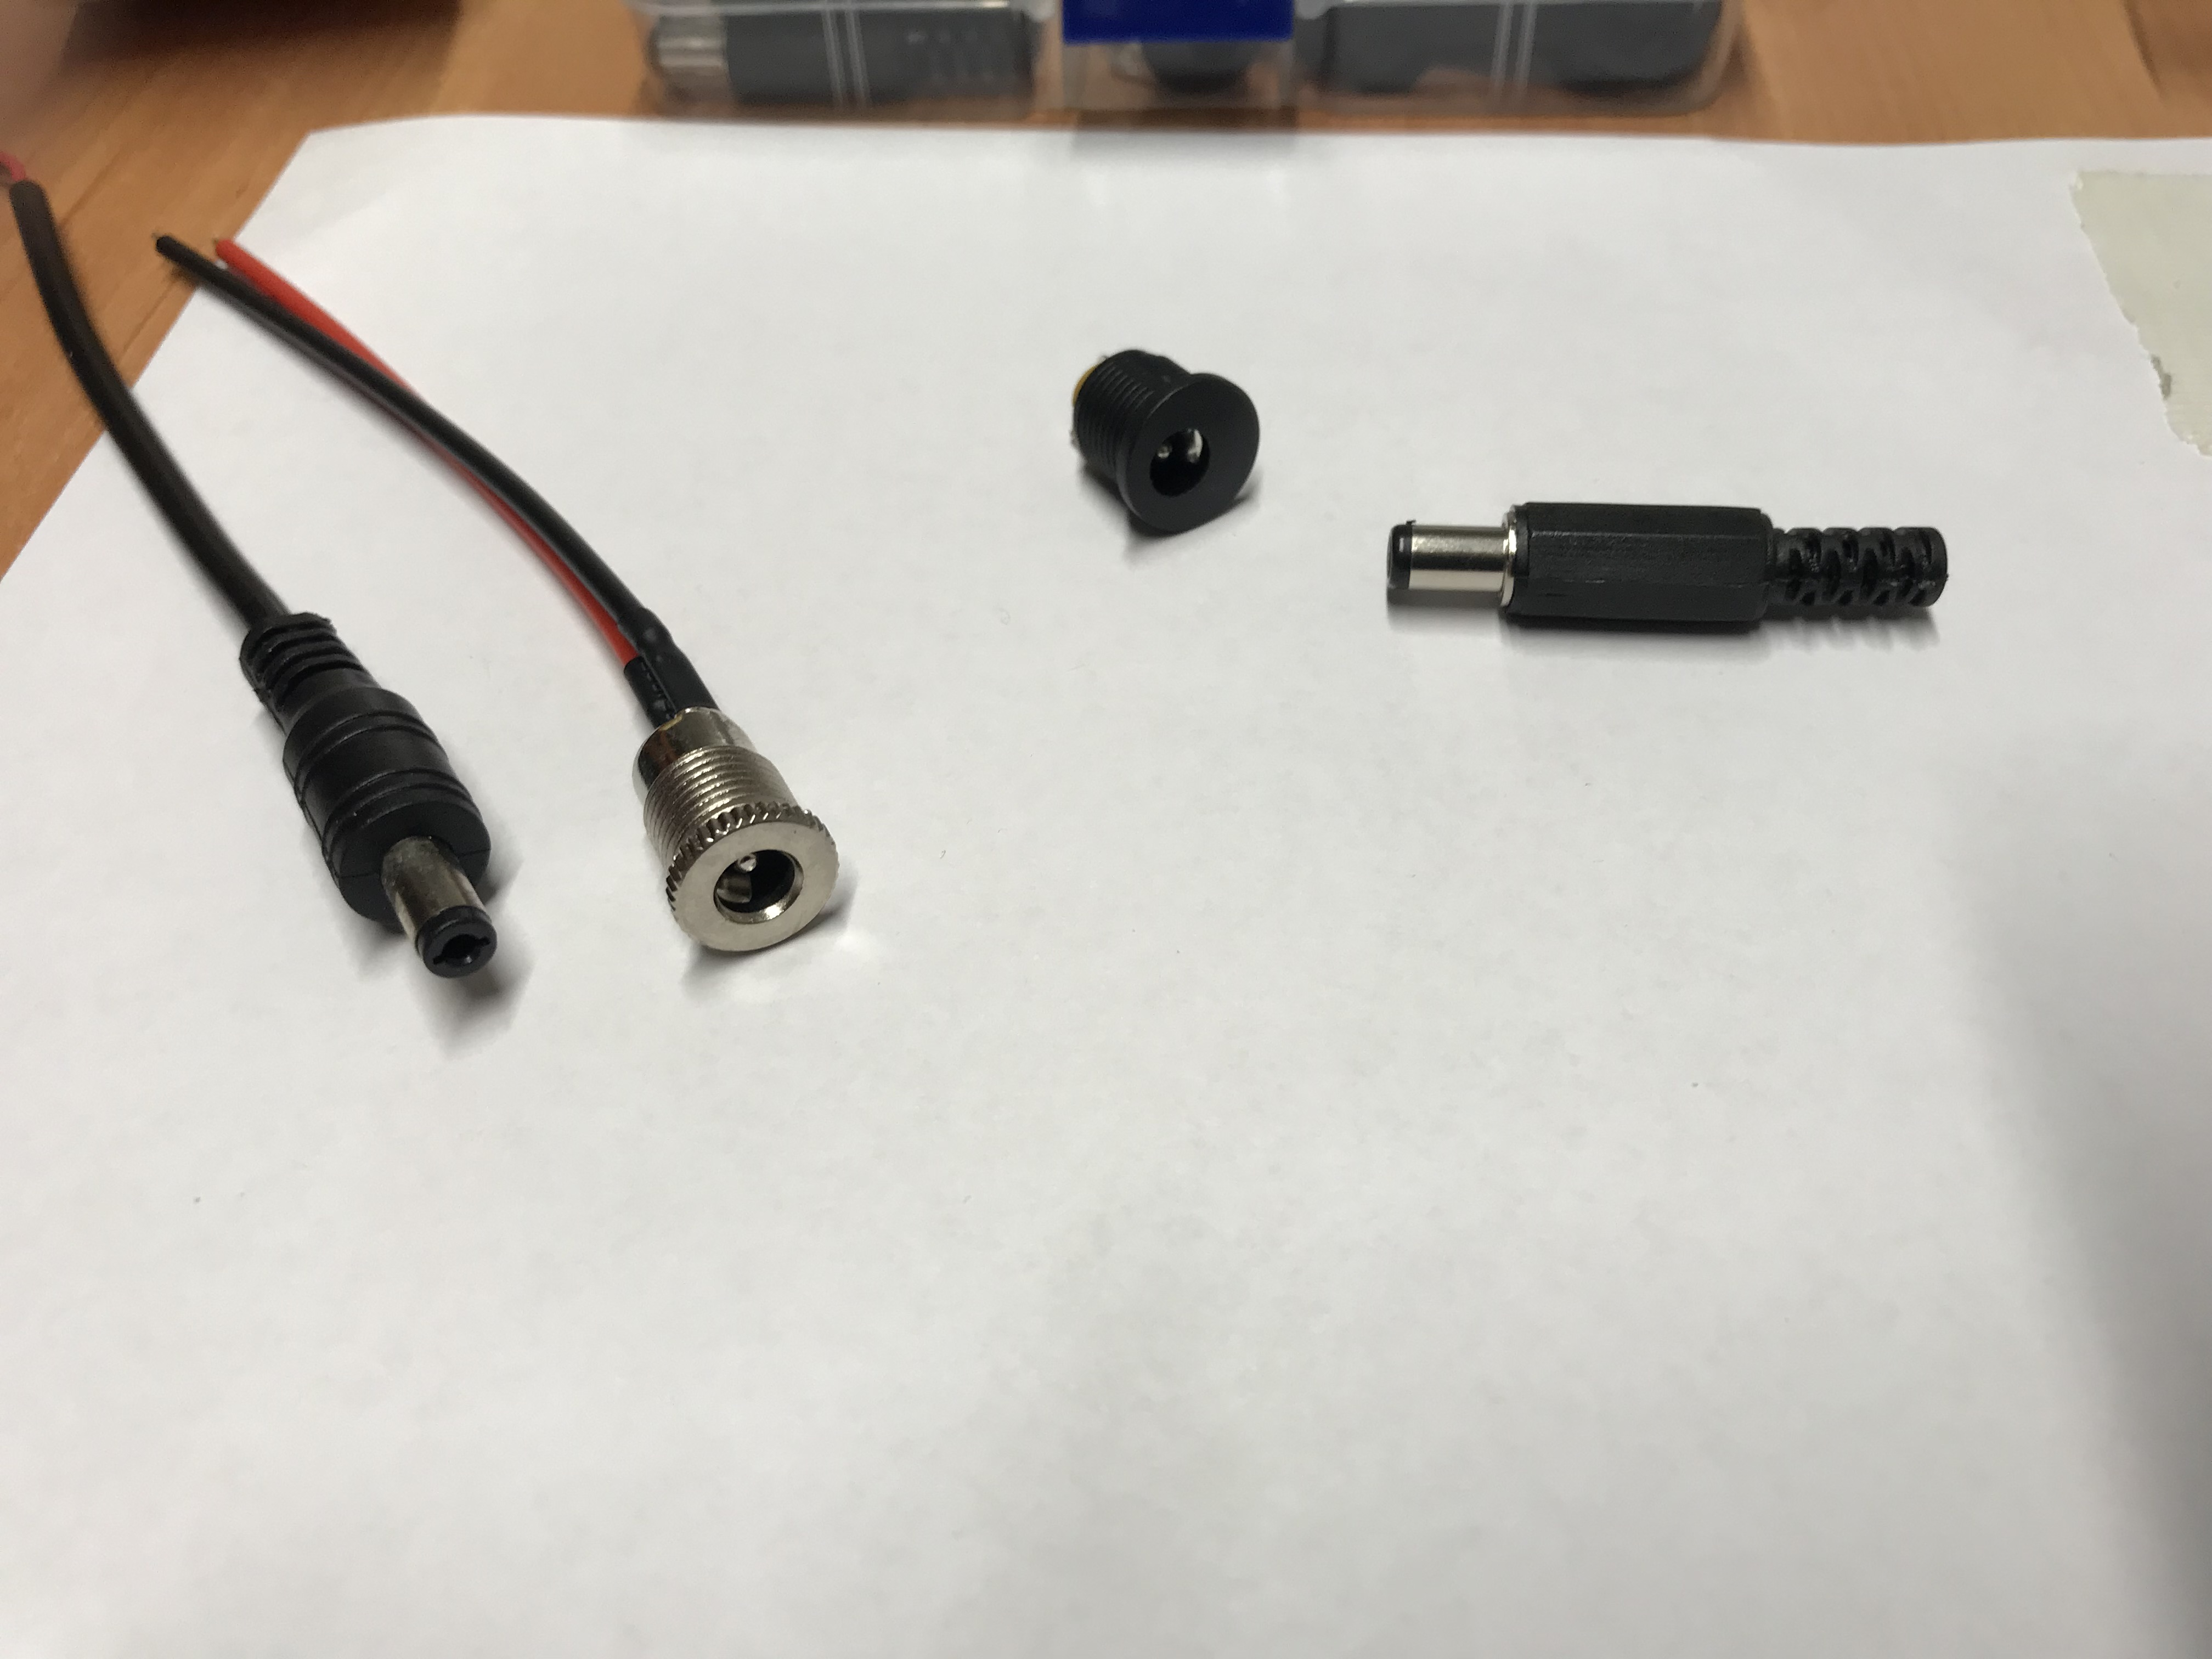
\includegraphics[scale=.05]{pictures/dcJack.jpg}};
            \end{scope}
        }{
            \draw (0,0) rectangle (3,1.5) ;
        }{Amazon}{Sin Id} {24V} {3A}
        \multirow{3}{*}{\makecell{Hembra \\ Socket}}
        \connectordata{
            \begin{scope}
                \clip (-1,-0.75) rectangle  +(2,1.5);
                \node[inner sep=0pt] at (-0.2,-1.7)
                    {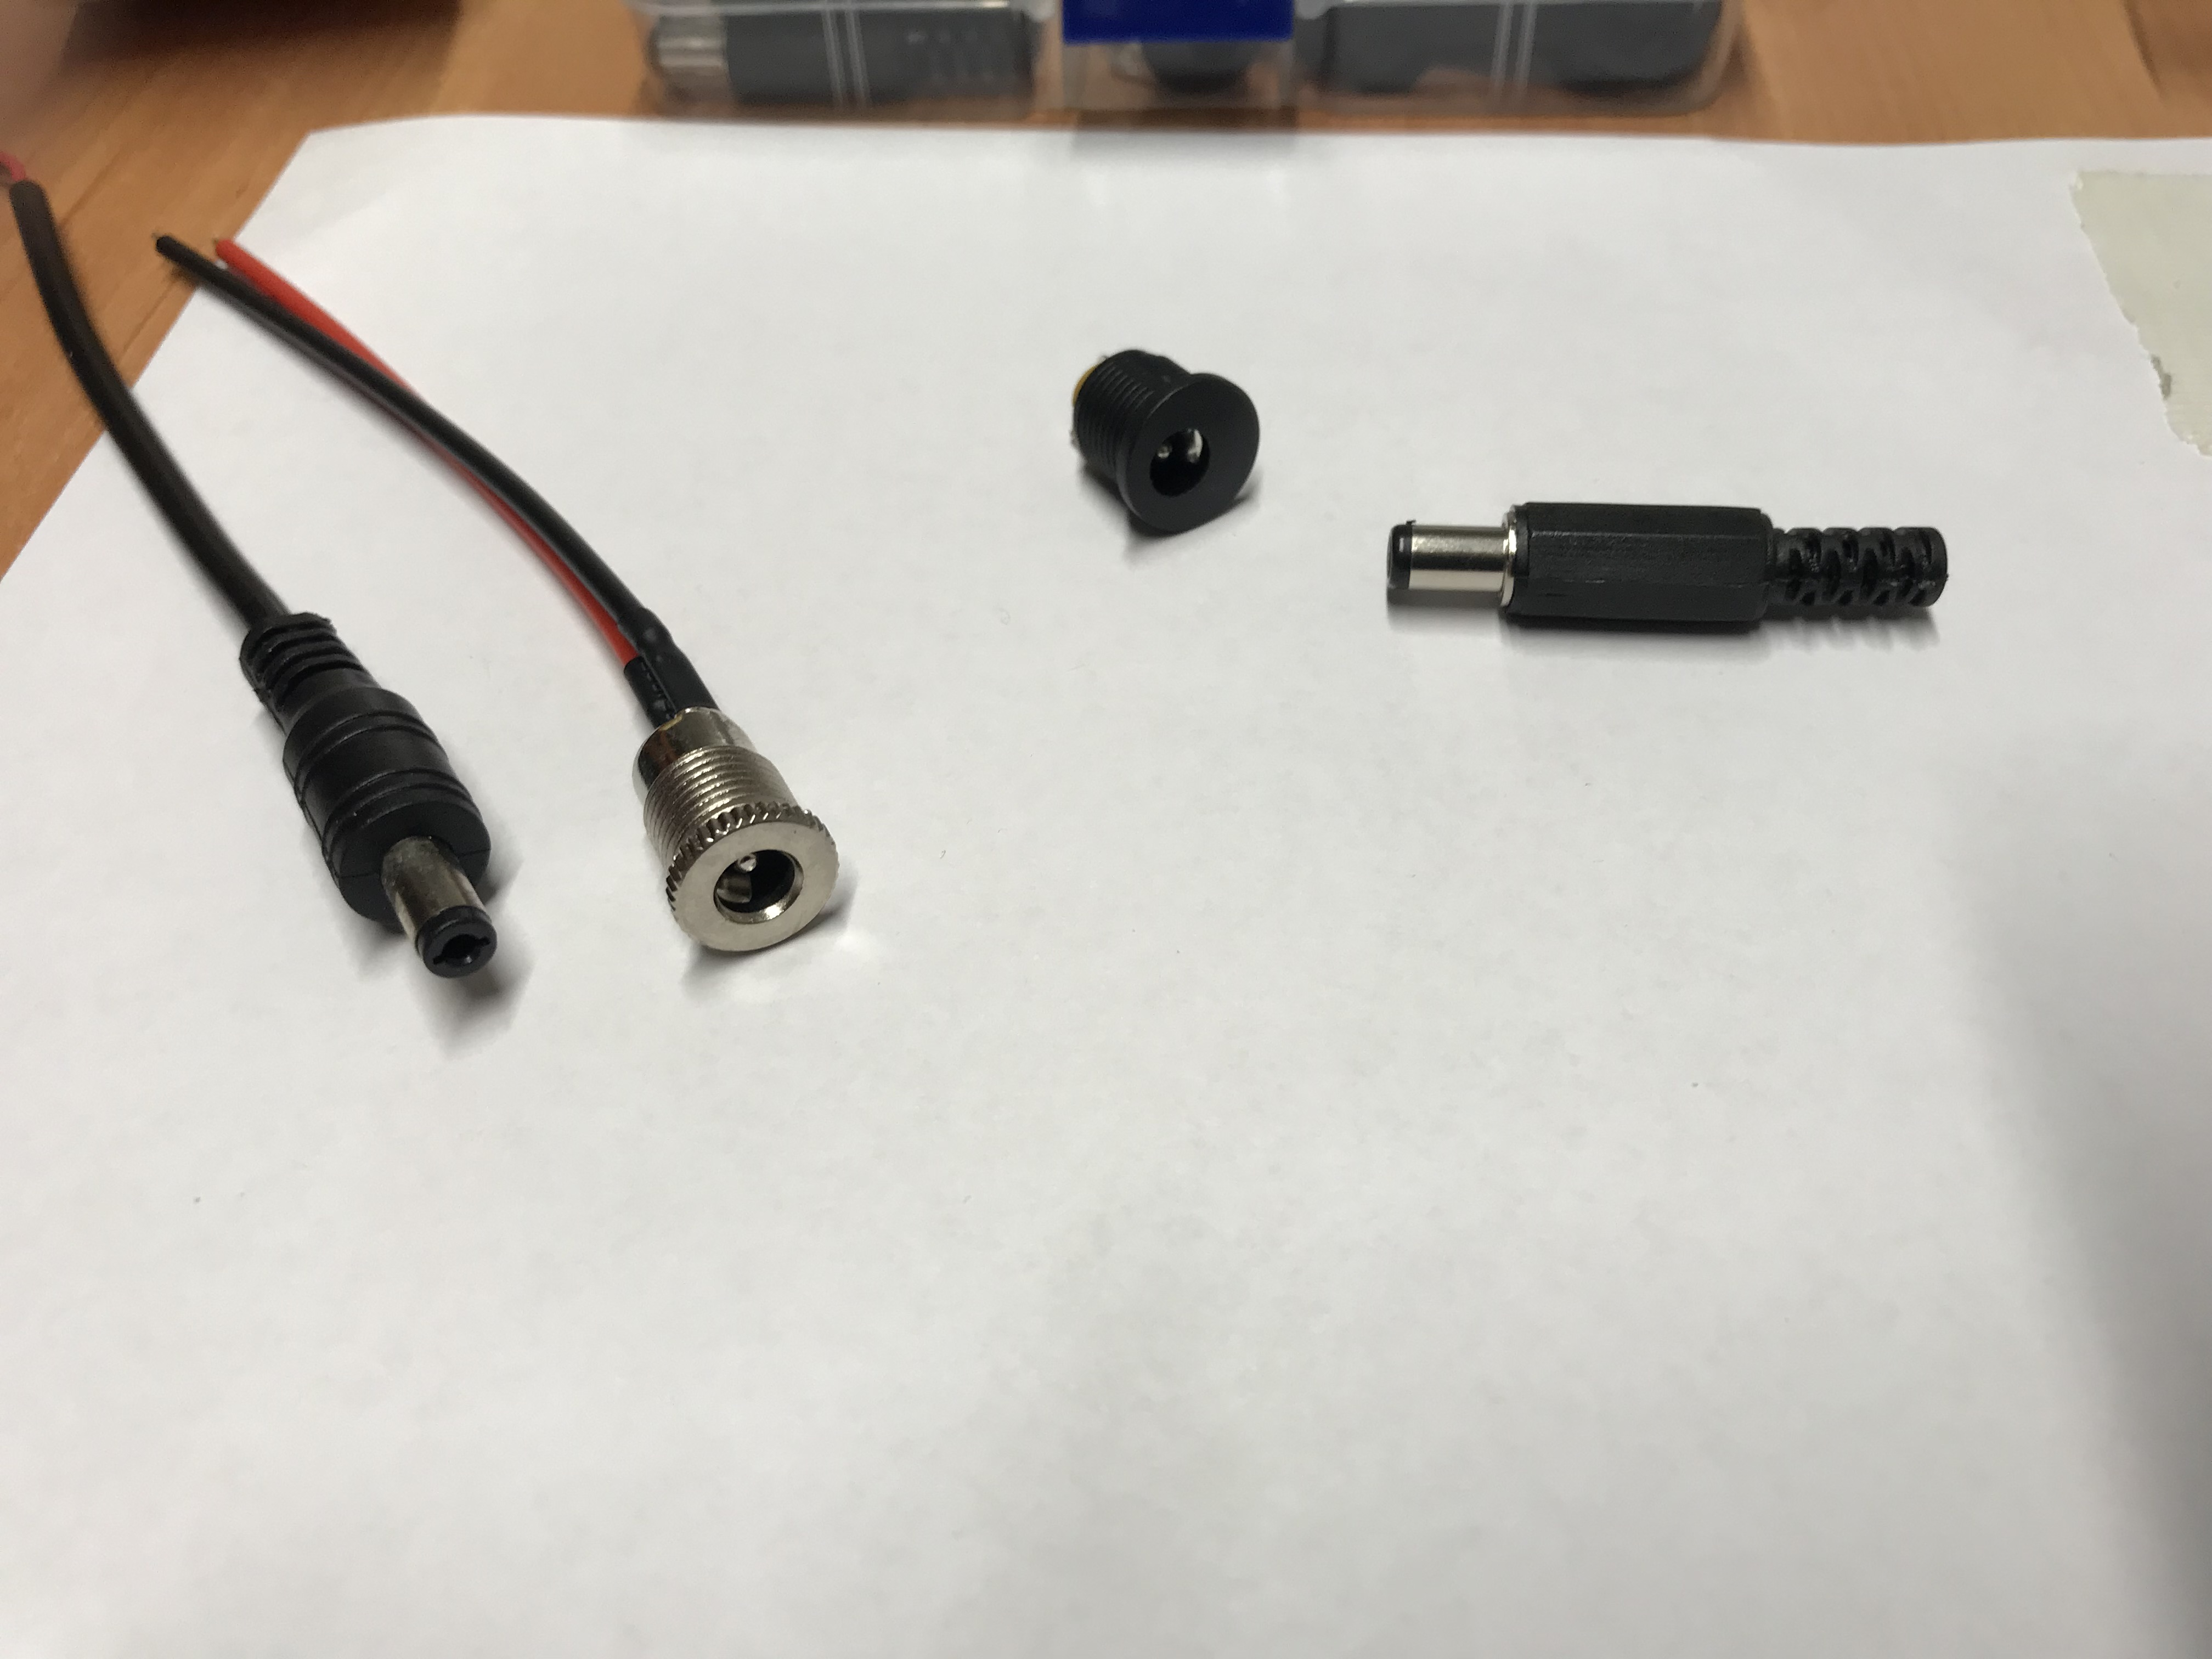
\includegraphics[scale=.07]{pictures/dcJack.jpg}};
            \end{scope}
        }{
            \draw (0,0) rectangle (3,1.5) ;
        }{Amazon}{Sin Id} {24V} {3A}

        \multicolumn{5}{|l|}{\makecell[l]{
            \tabitem Incluye tuerca para sujetar a panel \\
            \tabitem Incluye protector de goma
        }} \\
        \hline
    \end{tabular}
    \caption{Jack 2mm Amazon}
    \label{tab:DcJack1}
\end{table}

\begin{table}[H]
    \centering
    \renewcommand\theadfont{\bfseries}
    \setlength{\tabcolsep}{10pt}
    \renewcommand{\arraystretch}{1.5}

    \begin{tabular}{|c|c|c|c|c|}
        \beginConnectorTable{DC Jack 2mm}
        \multirow{3}{*}{\makecell{Macho \\ Plug}}
    
        \connectordata{
            \begin{scope}
                \clip (-1,-0.65) rectangle  +(2,1.3);
                \node[inner sep=0pt, rotate=60] at (1.3,2)
                    {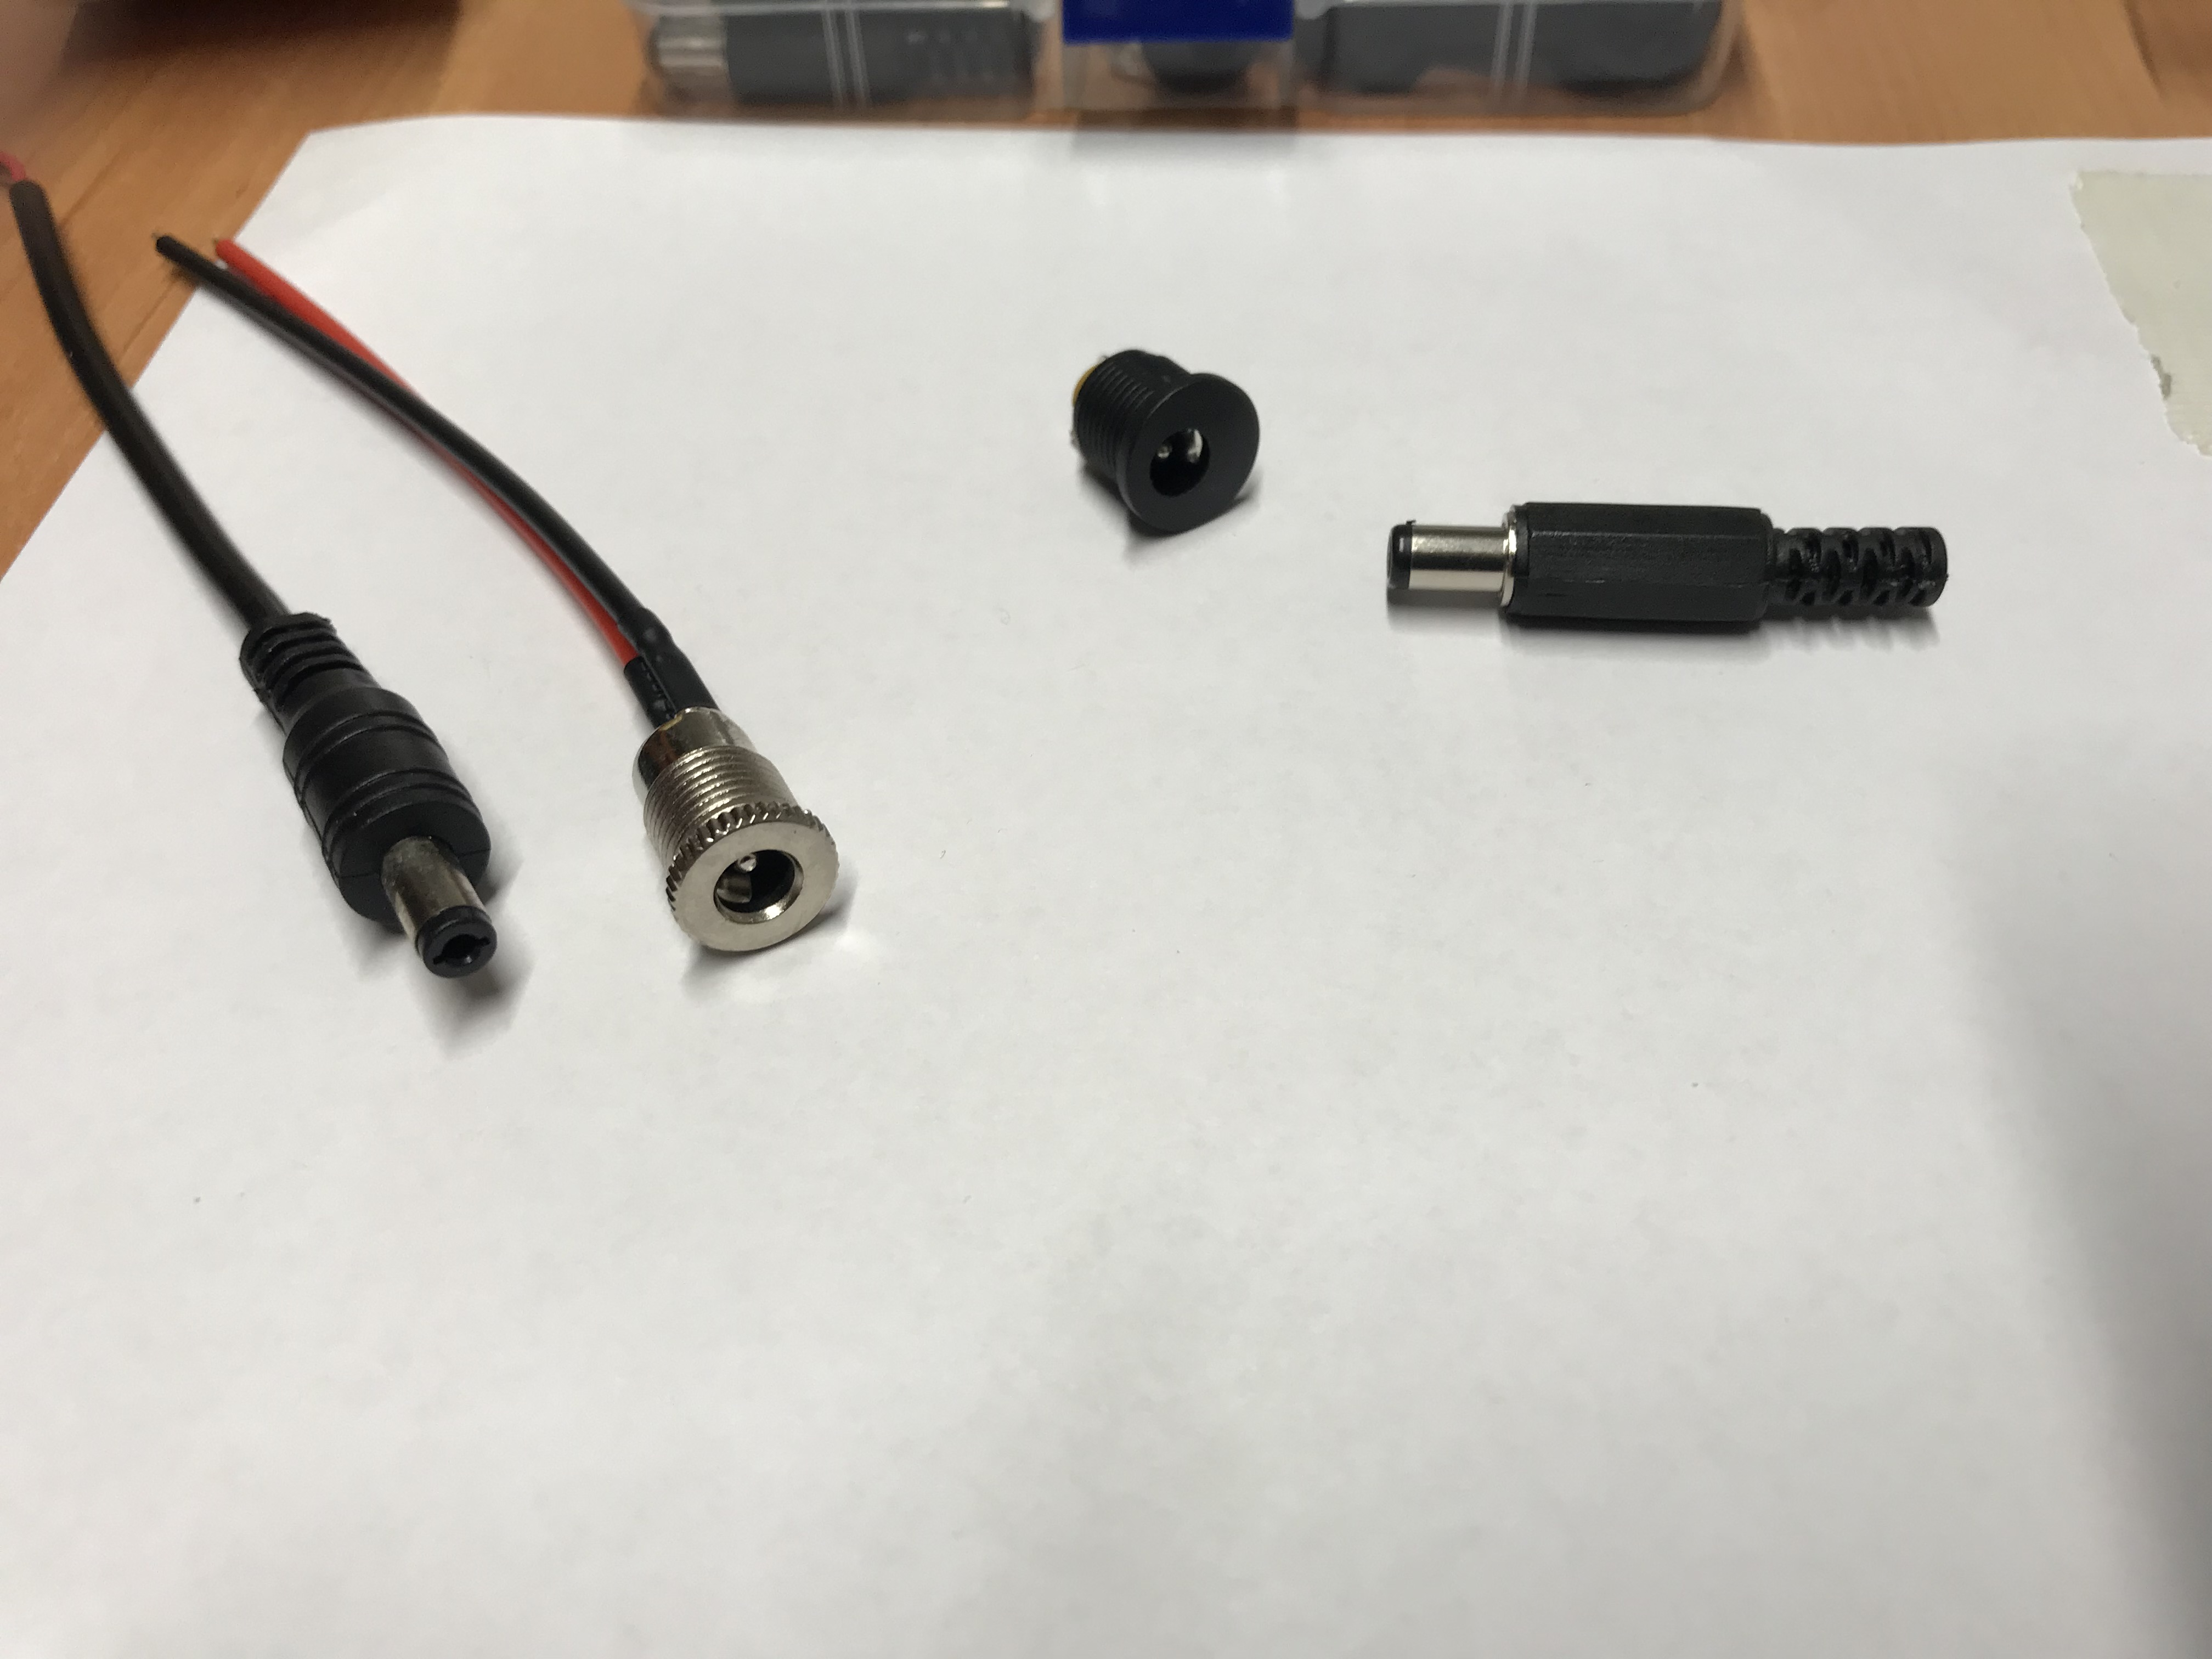
\includegraphics[scale=.05]{pictures/dcJack.jpg}};
            \end{scope}
           
        }{
            \draw (0,0) rectangle (3,1.5) ;
        }{Amazon}{Sin Id} {24V} {3A}
        \multirow{3}{*}{\makecell{Hembra \\ Socket}}
        \connectordata{
            \begin{scope}
                \clip (-1,-0.65) rectangle  +(2,1.3);
                \node[inner sep=0pt, rotate=60] at (0.9,1)
                    {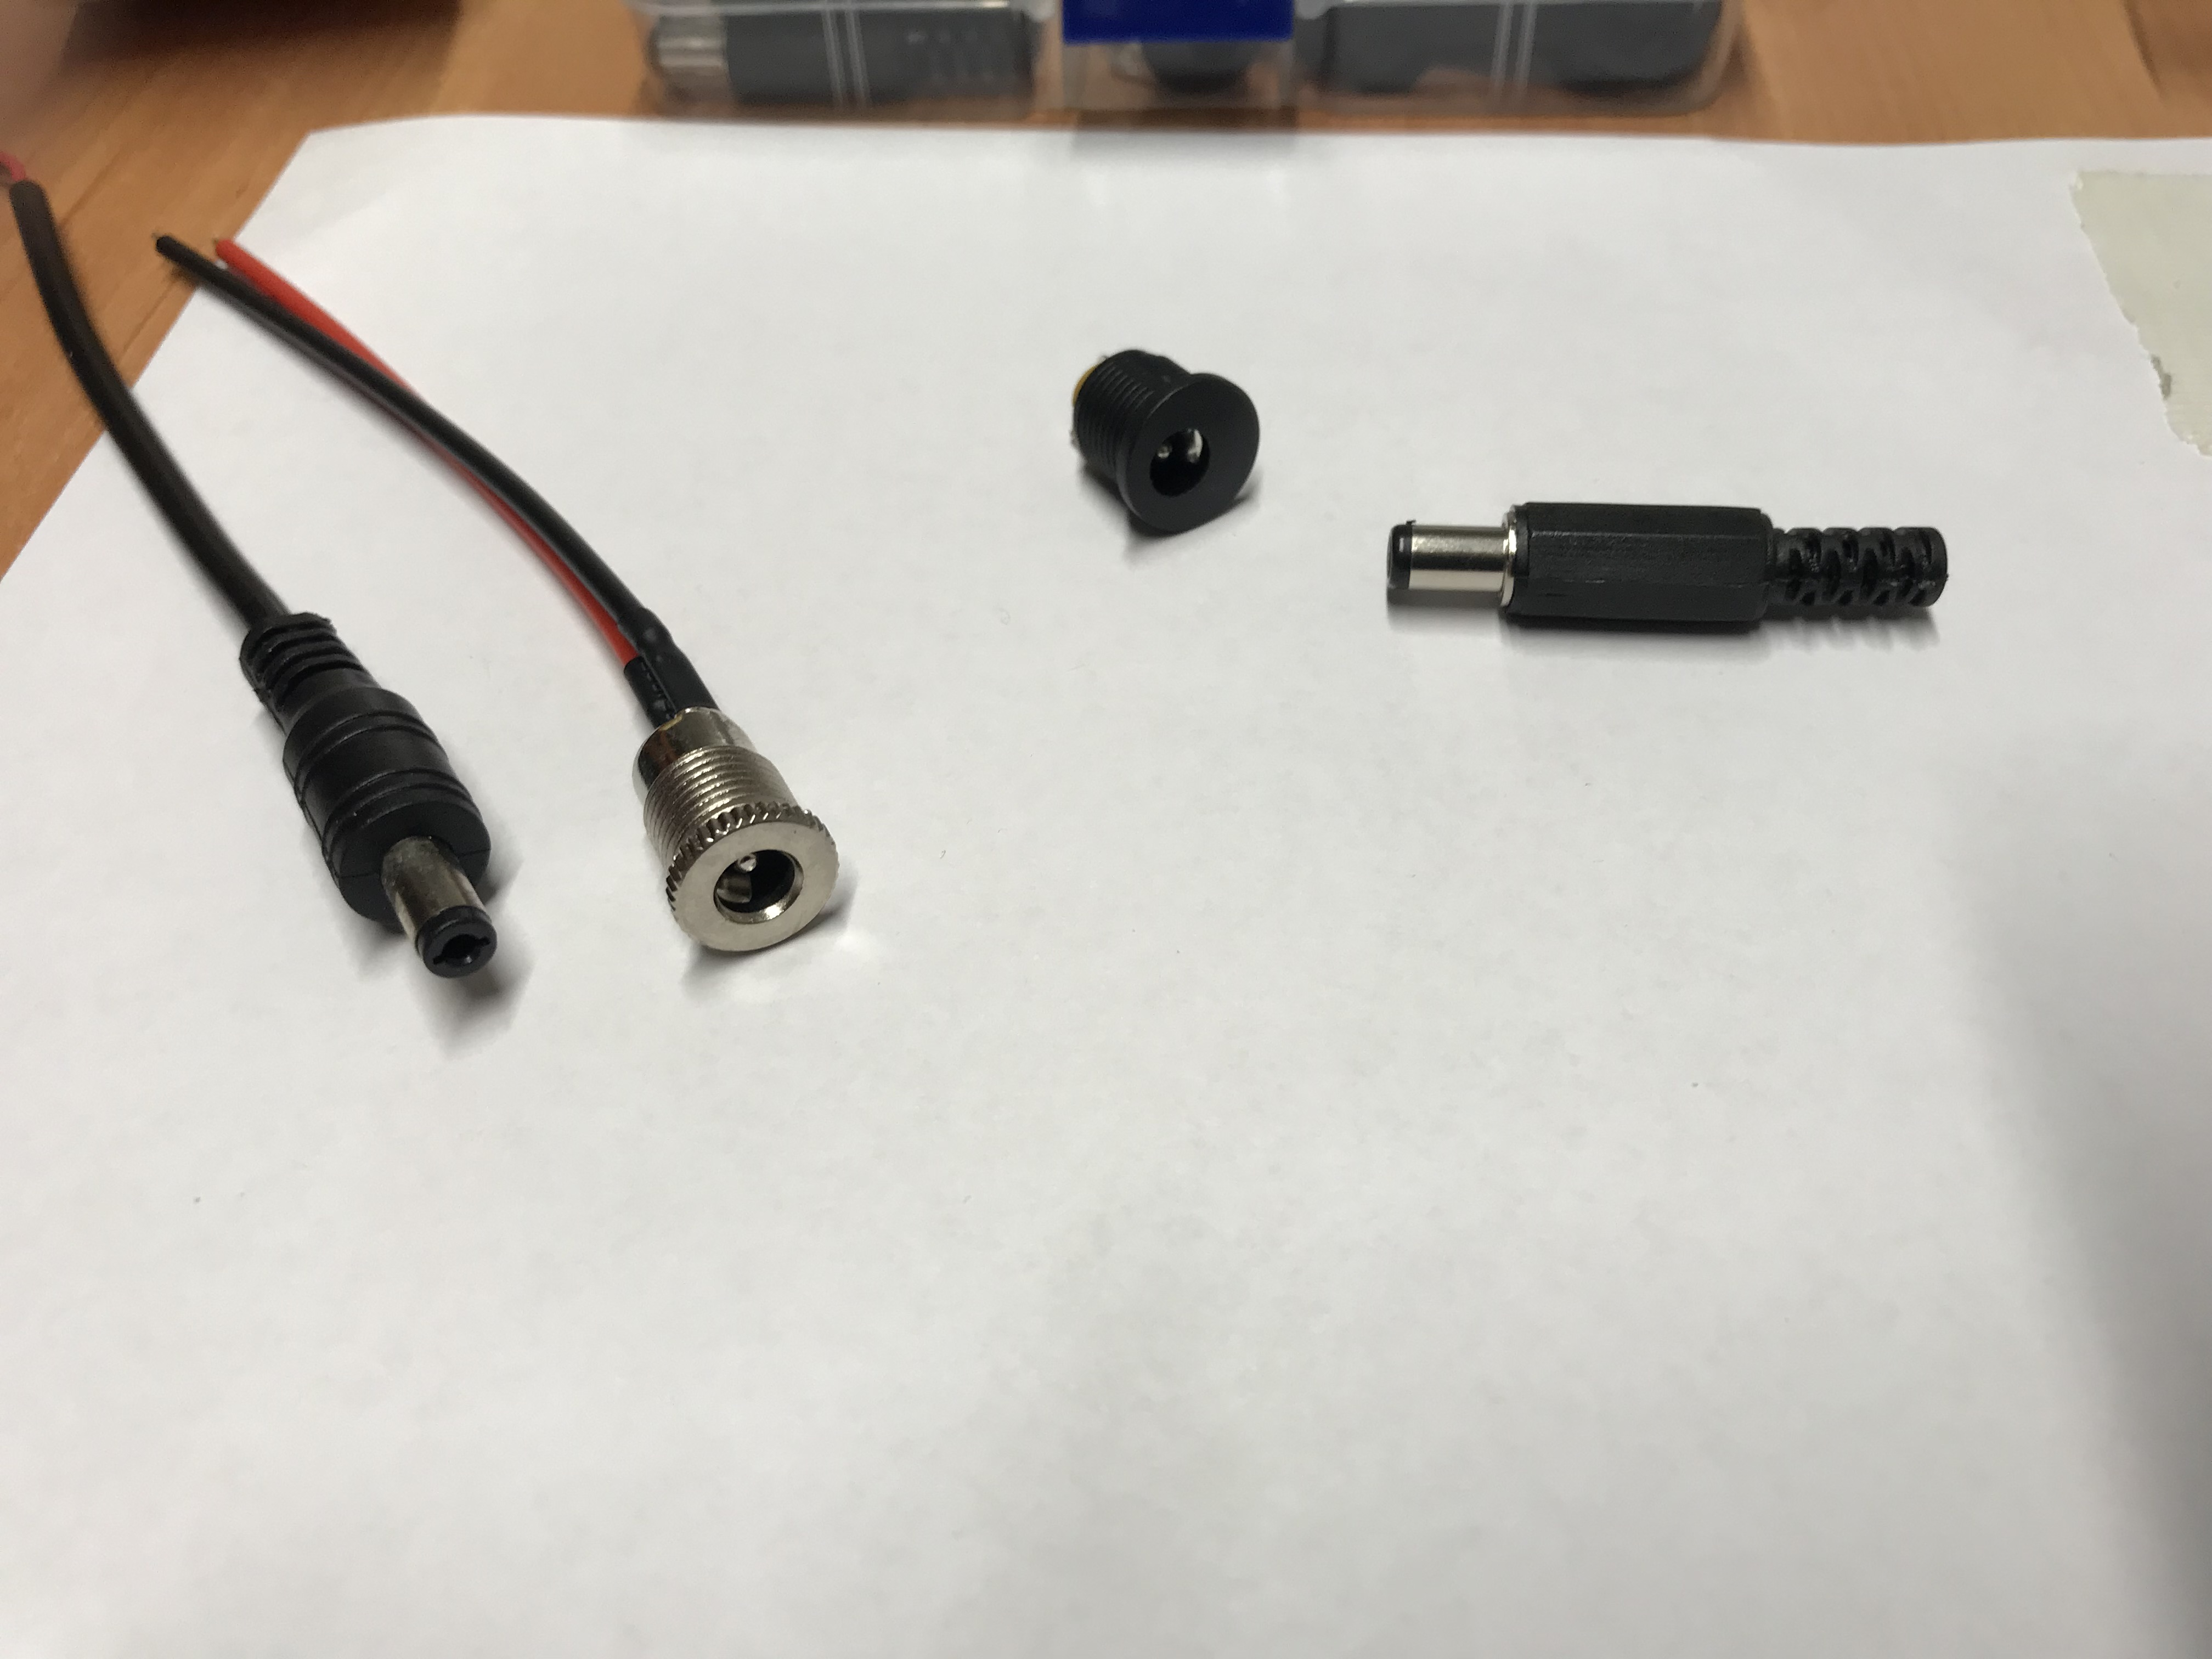
\includegraphics[scale=.05]{pictures/dcJack.jpg}};
            \end{scope}
        }{
            \draw (0,0) rectangle (3,1.5) ;
        }{Amazon}{Sin Id} {24V} {3A}

        \multicolumn{5}{|l|}{\makecell[l]{
            \tabitem Incluye tuerca para sujetar a panel \\
            \tabitem Es de metal conectado a (-) \\
            \tabitem Cables pre-soldados
        }} \\
        \hline
    \end{tabular}
    \caption{Jack 2mm Amazon}
    \label{tab:DcJack2}
\end{table}


\begin{table}[H]
    \centering
    \renewcommand\theadfont{\bfseries}
    \setlength{\tabcolsep}{10pt}
    \renewcommand{\arraystretch}{1.5}


    \begin{tabular}{c |c |c |c |c |}
        entrada & \thead[b]{item} & \thead[b]{Recomendado} & \thead[b]{Maximo} & \thead[b]{Con Bypass} \\ 
        \Xhline{5\arrayrulewidth}
%Entrada DCC
        \rowcolor{Melon!15}
        & Voltaje &14-20V & \multicolumn{2}{c|}{12-24V} \\
        \cline{2 - 5}
        \rowcolor{Melon!10} \cellcolor{Melon!15}
        \multirow{-2}{*}{DCC}&Corriente & 1A & 1.5A & 2A \\ \Xhline{3\arrayrulewidth}
%Entrada Jack
        \rowcolor{blue!15} & Voltaje & 12-20V & \multicolumn{2}{c|}{10-24V} \\
        \cline{2 - 5}
        \rowcolor{blue!10} \cellcolor{blue!15} \multirow{-2}{*}{ \makecell{ \cellcolor{blue!15} Jack\\ \cellcolor{blue!15} Terminal}} & Corriente & 1A & 1.5A & 3A \\
        \Xhline{5\arrayrulewidth}
    \end{tabular}
    \caption{Limites de entrada}
    \label{tab:limiteEntrada}
\end{table}
\end{document}